% JUMP TO LINE 60, 75
% \documentclass[preview, margin=0.6in]{standalone}
\documentclass{article}
\usepackage[letterpaper,portrait,top=0.4in, left=0.6in, right=0.6in, bottom=1in]{geometry}

\usepackage{amsmath, amsfonts, amsthm, amssymb}
\usepackage{setspace}
\usepackage{sectsty}
\usepackage{graphicx}
\usepackage{parskip}

\newtheorem{thm}{Theorem}[section]
\newtheorem{defn}{Definition}[section]
\newtheorem{lemma}{Lemma}[section]
\newtheorem{corthm}{Corollary}[thm]
\newtheorem{cordefn}{Corollary}[defn]
\newtheorem{remark}{Remark}[section]
\newtheorem{prop}{Proposition}[section]
\newtheorem{example}{Example}[section]

\title{\vspace*{-40pt}Graph Theory}
\author{Jayden Li}
\date{\today}

\begin{document}
\setstretch{1.25}
\fontsize{12pt}{12pt}\selectfont
\sectionfont{\fontsize{16}{16}\selectfont}
\subsectionfont{\fontsize{14}{14}\selectfont}
\maketitle

\section{Graph Basics}
\begin{defn}[Graph]
	A graph $G$ is a triple containing the vertex set $V(G)$, the edge set $E(G)$ and a relationship between vertices and edges called the endpoints.
\end{defn}
The endpoints are often defined by means of an image.

\begin{defn}[Loop]
	A loop is an edge whose endpoints are equal.
\end{defn}

\begin{defn}[Multiple edges]
	Multiple edges are edges with the same endpoints.
\end{defn}

\begin{defn}[Simple graph]
	A simple graph is a graph without loops or multiple edges.
\end{defn}

The edges of a simple graph can be specified with only the vertices: an edge $e=uv$ where $u,v\in V(G)$.

\begin{defn}[Adjacency]
	If there exists an edge $e\in E(G)$ with endpoints $u$ and $v$, then $u$ and $v$ are adjacent.
\end{defn}

\begin{defn}[Null graph]
	A null graph $G$ is a graph such that $\left|V(G)\right|=\left|E(G)\right|=0$.
\end{defn}

\begin{defn}[Complement of a graph]
	The complement of a simple graph $G$, denoted $\overline G$, is a simple graph such that $uv\in E(\overline G)$ if and only if $uv\not\in E(G)$.
\end{defn}

\begin{defn}[Clique]
	A clique is a set of vertices such that each vertex is adjacent to all other vertices.
\end{defn}

\begin{defn}[Independent set]
	An independent set is a set of vertices such that each vertex is not adjacent to all other vertices.
\end{defn}

\begin{defn}[Bipartite graph]
	A bipartite graph is a graph that can be divided into two disjoint and independent sets $U,V$ called partites, so that each edge in $E(G)$ are between a vertex in $U$ and a vertex in $V$.
\end{defn}
A graph is bipartite if and only if there are no odd cycles.

\begin{defn}[Path]
	A path is a simple graph whose edges join a sequence of vertices, and so that the vertices can be ordered in a list.
\end{defn}

\begin{defn}[Cycle]
	A cycle is a graph with an equal number of edges and vertices, so that the vertices can be placed into a circle.
\end{defn}

\begin{defn}[Subgraph]
	A graph $H$ is a subgraph of $G$ if $V(H)\subseteq V(G)$ and $E(H)\subseteq E(G)$, and is denoted $H\subseteq G$.
\end{defn}

\begin{defn}[Connectedness]
	A graph $G$ is connected if for all vertices $u,v\in V(G)$, there exists a path between $u$ and $v$. A graph $G$ is not connected if there exists two vertices $u,v\in V(G)$ such that no path exists between $u$ and $v$.
\end{defn}

\begin{defn}[Incidence and Degree]
	If $u\in V(G)$ is an endpoint of an edge $e\in E(G)$, then $u$ and $e$ are incident. The degree of a vertex is the number of incident edges.
\end{defn}

\begin{defn}
	$P_n$ denotes a path with $n$ vertices and $n-1$ edges. $C_n$ denotes a cycle with $n$ vertices and $n$ edges.
\end{defn}

\begin{defn}[Completeness]
	A graph is complete if every vertex is adjacent to every other vertex. A complete graph with $n$ vertices is denoted $K_n$.
\end{defn}

\begin{defn}[Complete bipartite graph]
	A complete bipartite graph is a bipartite graph such that two vertices are adjacent if and only if they are in different partite sets, and is denoted $K_{r,s}$ where $r,s$ are the size of each bipartite set.
\end{defn}

\begin{defn}[Regularity]
	A $k$-regular graph is one where every vertex is of degree $k$.
\end{defn}

\section{Petersen graph}

\begin{defn}[Petersen graph]
	The Peterson graph is a simple graph whose vertices are 2-element subsets of a 5-element set and whose edges are the pairs of disjoint 2-element subsets.
\end{defn}
\begin{center}
	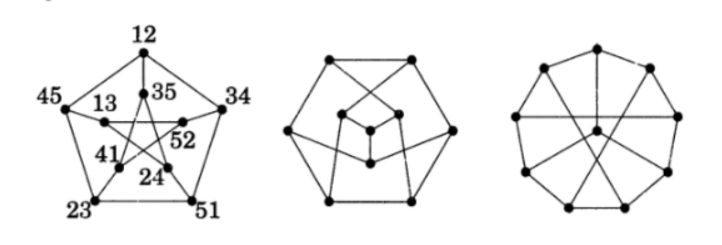
\includegraphics[width=0.6\linewidth]{petersen.png}
\end{center}
Assign each point a pair of numbers. There are $\binom 52=10$ vertices, and connect two points with an edge if they do not share any number. Every vertex is degree $3$ so the Petersen graph so it is $3$-regular.

\begin{prop}
	If two vertices are nonadjacent in the Petersen graph then they have exactly one common neighbor.
\end{prop}

\begin{defn}[Girth]
	The girth of a graph with a cycle is the length of its shortest cycle. A graph with no cycle has infinite girth.
\end{defn}
\begin{cordefn}
	The Petersen graph has girth $5$.
\end{cordefn}
There cannot be a $3$-cycle including points $ab$ and $cd$, because another point connected to both $ab$ and $cd$ must not share any elements in the $5$-element set. But there is only one element in the set that is not $a,b,c,d$, so no such point can exist.

There cannot be a $4$-cycle including points $ab$ and $bc$ (share $b$ because they are not connected), because there cannot exist two other points that share one element in the set in order to not be connected.

\section{Matrix Representations}
\begin{defn}[Adjacency matrix]
	The adjacency matrix $A(G)$ of a graph with $n$ vertices $\{v_1,v_2,\ldots,v_n\}$ is an $n\times n$ matrix in which the entry $a_{ij}$ is the number of edges in $G$ with endpoints $v_i,v_j$.
\end{defn}
If an edge has endpoints $v_i$ and $v_j$, it would add to both entries $a_{ij}$ and $a_{ji}$, so an adjancency matrix must be symmetric.

\begin{defn}[Incidence matrix]
	The incidence matrix $M(G)$ of a graph with $n$ vertices $\{v_1,v_2,\ldots v_n\}$ and $m$ edges $\{e_1,e_2,\ldots,e_m\}$ is an $n\times m$ matrix in which the entry $m_{ij}$ is 1 if $v_i$ is an endpoint of edge $e_j$, and $0$ if not.
\end{defn}

\section{Isomorphism}
An equivalence relation is a relation between two sets that is reflexive, symmetric and transitive.

\begin{defn}[Isomorphism]
	An isomorphism from a simple graph $G$ to a simple graph $H$ is a bijection $f:V(G)\to V(H)$ such that $uv\in E(G)$ if and only if $f(u)f(v)\in E(H)$. Isomorphism is denoted as $G\cong H$.
\end{defn}

A graph $G$ is isomorphic to a graph $H$ if and only if we can permute the columns and rows of the adjacency matrix of $G$ to create the adjacency matrix of $H$.

An isomorphism class is an equivalence class:
\begin{itemize}
	\item Reflexivity: A graph $G$ is isomorphic to itself.
	\item Symmetry: If $G$ is isomorphic to $H$, then $H$ is isomorphic to $G$.
	\item Transitivity: If $G$ is isomorphic to $H$, and $H$ is isomorphic to $K$, then $G$ is isomorphic to $K$.
\end{itemize}

Disproving bipartiteness: find an odd cycle. If one exists, one point in the cycle will be connected to both set of points.

To prove an isomorphism, we identify a bijective mapping that preserves all adjacencies, and is often done by establishing a labelling.

To prove graphs are not isomorphic, demonstrate they contradict each other with features.

\begin{thm} \label{thm:isomorphiccomplement}
	$G\cong H$ if and only if $\overline G \cong \overline H$.
\end{thm}

\begin{proof}[Proof of Theorem \ref{thm:isomorphiccomplement}]
	Suppose $G$ and $H$ are isomorphic, and let $f$ be a bijection such that $uv\in E(G)$ if and only if $f(u)f(v)\in E(H)$. Thus $uv\not\in E(G) \iff f(u)f(v)\not\in E(H)$.

	By the definition of the graph complement, $uv\in E(\overline G)$ if and only if $uv\not\in E(G)$, and $uv\in E(\overline H)$ if and only if $uv\not\in E(H)$. So:
	\begin{equation*}
		uv\not\in E(G)
		\iff f(u)f(v)\not\in E(H)
		\iff (uv\in E(\overline G)
		\iff f(u)f(v)\in E(\overline H))
	\end{equation*}
	Thus, $\overline G$ is isomorphic to $\overline H$.

	Now we prove the only if case: if $\overline G\cong \overline H$, then $G\cong H$.
	\begin{equation*}
		\overline G\cong \overline H
		\implies G=\overline{\overline G}\cong \overline{\overline H}=H
	\end{equation*}
	So $G$ is isomorphic to $H$.
\end{proof}

\begin{defn}[Self-complementary]
	A graph is self-complementary if it is isomorphic to its complement. 
\end{defn}
The graph $P_4$ is isomorphic to its complement $\overline{P_4}$.

\section{Decomposition}
\begin{defn}[Decomposition]
	A decomposition of a graph is a list of subgraphs such that each edge appears in exactly one subgraph in the list.
\end{defn}

\begin{thm}
	An $n$-vertex graph $H$ is self-complementary if and only if $K_n$ has a decomposition consisting of two copies of $H$.
\end{thm}

For example, $K_5$ can be decomposed into two $5$-cycles. If we placed the vertices in a pentagon and drew the edges, there are two $5$-cycles: the outer pentagon and the inner $5$-pointed star. So we know the $5$-vertex cycle $C_5$ is self-complementary.

To prove a graph can be decomposed, propose the subgraphs.

\end{document}
